\chapter{Load Testing}
We used Tsung~\cite{tsung} framework for load testing. We designed a \textit{generic workflow} which was able to capture the usual activities of a user while covering most, if not all, features of our website. We ran most of our tests on this generic workflow. Testing on the generic workflow gave us a rough idea on the overall performance of our website and possible bottlenecks. Later we created \textit{specific workflow} separating out the portions that we thought might be causing the greatest bottlenecks. We ran our tests on this specific workflow before and after optimization to verify that this was indeed the workflow that was causing the bottlenecks and that these have been remediated by the optimizations. Unless otherwise specified, all the tests documented in this report were run on a C5 large app server and a m4 large database server. The optimizations described in this section are incremental, that is, stacked over the previous optimization.

\section{Generic Workflow}\label{sec:generic-workflow}
In this workflow, at first a user logs in to the website. The user waits for a time between zero and two seconds, visits the games index page, and then waits again for a time between zero and one second. Then the user randomly visits a game page, waits for a time between zero and two seconds, comments on that game and then logs out. This concludes the first sessions of our workflow. 

In the second session, a user browses to the search page, searches for games by name, waits for a time between zero and one second, visits a random games page, waits for a time between zero and two seconds, searches for games by number of backgrounds, waits for a time between zero and two seconds, and visits a random game page. 

In the third session, a user browses to the gamers index page, waits between zero and one second, randomly gets a game, waits between zero and one second, browses to the genres page, waits between zero and one second, and finally browses to the companies page.

In the fourth session, a user browses to the signup page, waits for zero to three seconds, submits the form, waits for zero to one second, visits the games index page, waits for zero to one second, and finally likes/dislikes a random game.

For this workflow we had four arrival phases, the arrival rate being doubled at each consecutive phase and the very first one having an arrival rate of two users per second. Figure~\ref{fig:generic1} and ~\ref{fig:generic2} illustrate all the four sessions with the help of toned down sequence diagrams.

\begin{figure}
\subfloat[First session.]{%
  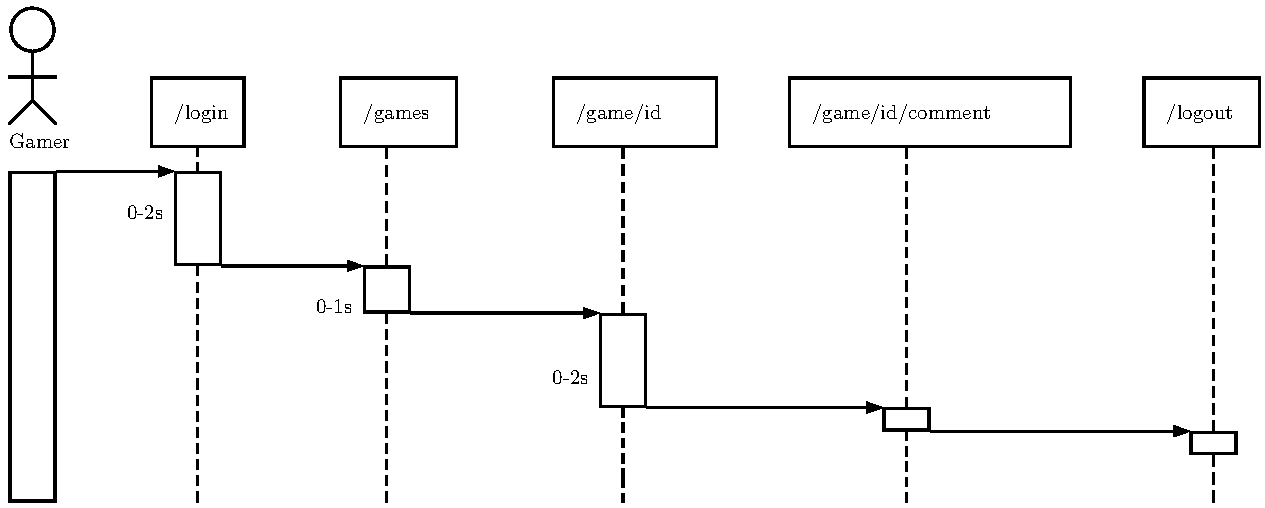
\includegraphics[clip,width=\columnwidth]{images/generic-1}%
}

\subfloat[Second session.]{%
  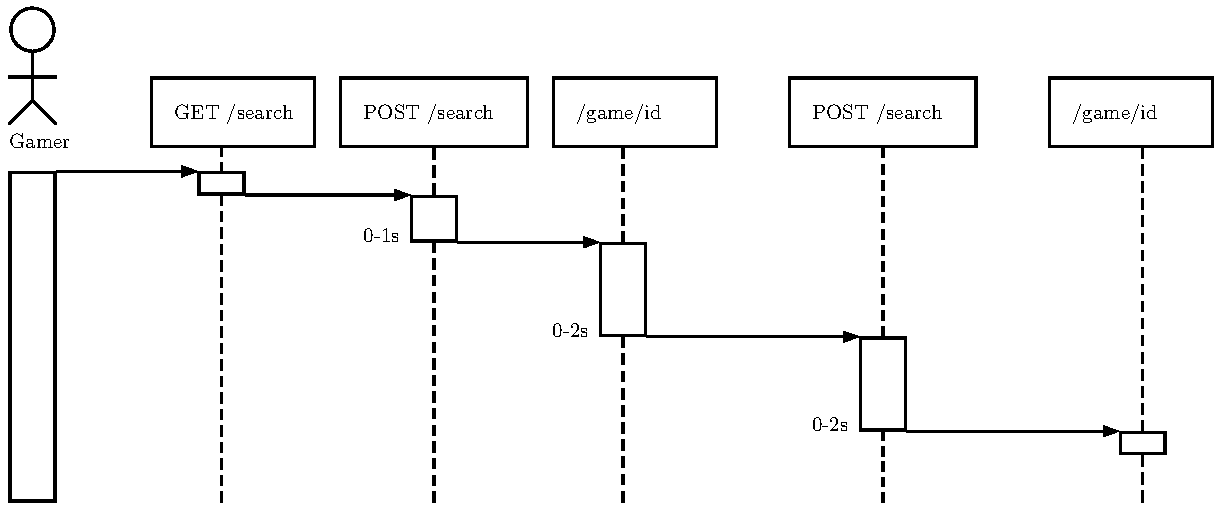
\includegraphics[clip,width=\columnwidth]{images/generic-2}%
}
\caption{First and second sessions of generic workflow.}\label{fig:generic1}
\end{figure}

\begin{figure}
\subfloat[Third session.]{%
  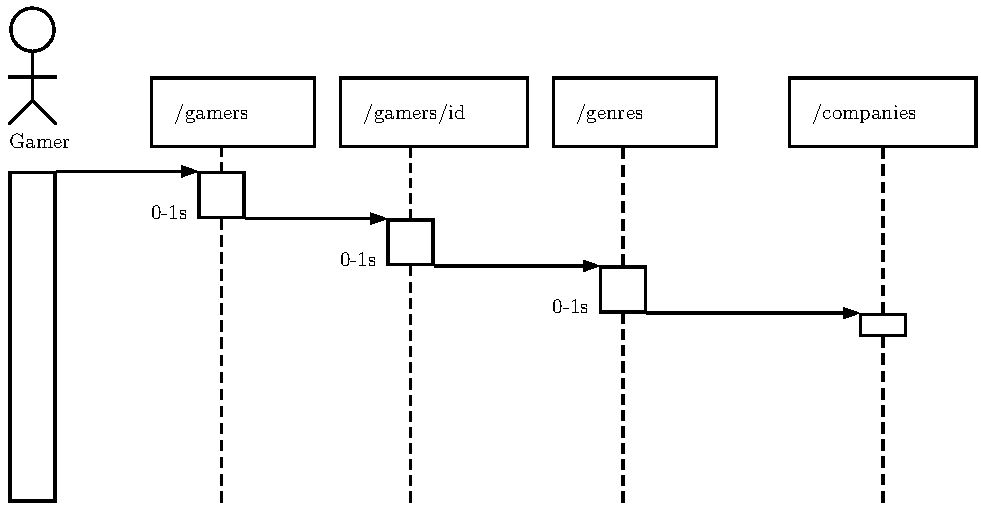
\includegraphics[clip,width=\columnwidth]{images/generic-3}%
}

\subfloat[Fourth session.]{%
  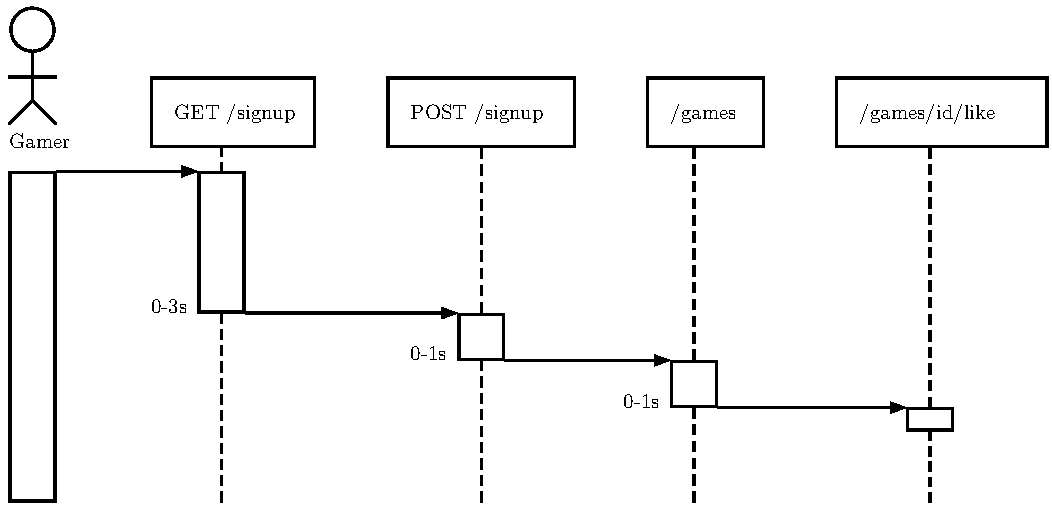
\includegraphics[clip,width=\columnwidth]{images/generic-4}%
}
\caption{Third and fourth sessions of generic workflow.}\label{fig:generic2}
\end{figure}

\section{Specific Workflow}\label{sec:specific-workflow}
It came to our observation that the number of sql queries being invoked in a couple of pages (index page of genres and companies) was higher than normal. We hypothesized optimizing the query in some way might improve our response time. Just to verify our hunch, we came up with a specific workflow and tested that before and after optimization. The exact optimization has been discussed in a later section.

In this workflow, a user hits the index page for games, followed by the index pages of genres and companies. For this workflow we had four arrival phases, the arrival rate being doubled at each consecutive phase and the very first one having an arrival rate of two users per second. Figure~\ref{fig:specific} illustrates the specific workflow with the help of a toned down sequence diagram.

\begin{figure}
	\centering
	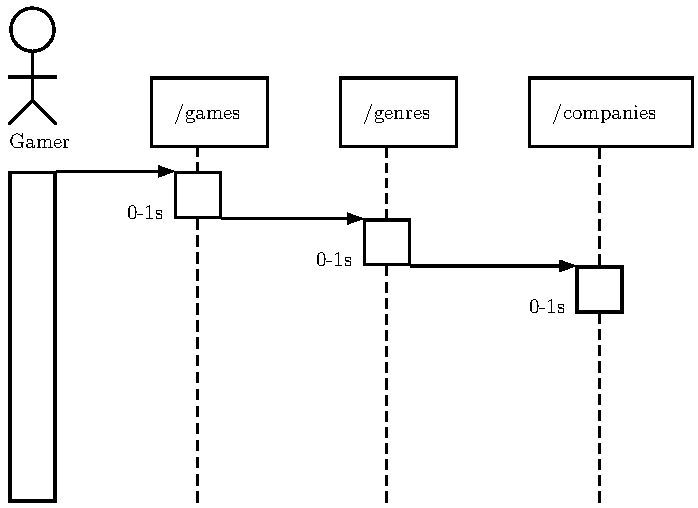
\includegraphics{images/specific}
	\caption{Specific workflow.}\label{fig:specific}
\end{figure}

\section{Optimization: AJAX}
We observed a huge number of 5xx response codes the first time our application was tested using the generic workflow. A quick look at the rails log revealed that for every game showed in the index page, a query was executed to get its likes/dislikes. Instead of showing this information automatically, we decided to invoke an AJAX request on hover over ``stats'' text. It was observed that this increased the number of 200 codes and decreaed the number of 5xx codes. Figure~\ref{fig:numcodes} shows the total number of 200 and 5xx codes over time for deployment without and with AJAX.
\begin{figure}
	\centering
	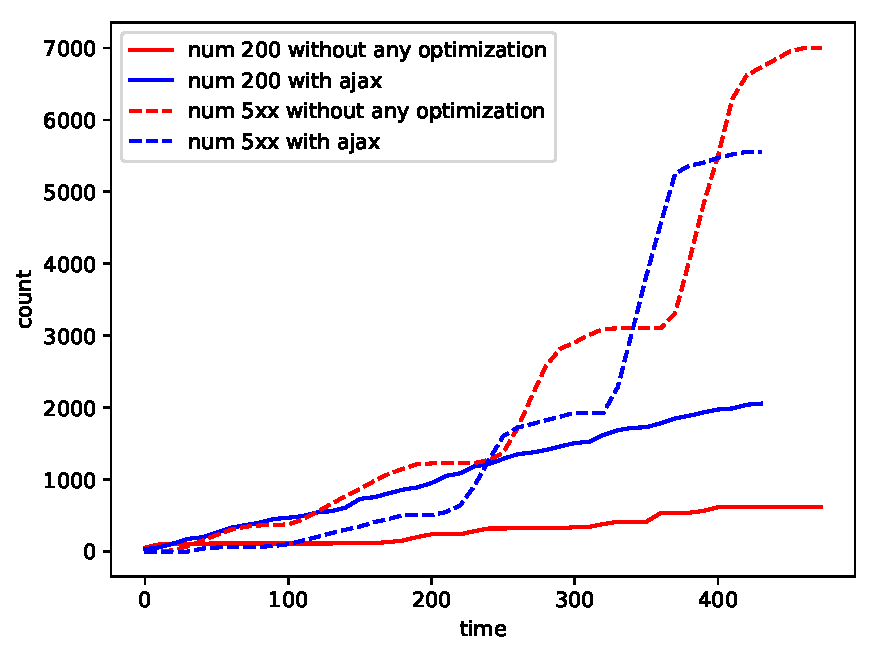
\includegraphics[width=0.8\textwidth]{images/without-any-optimization-with-ajax.pdf}
	\caption{HTTP response counts with and without ajax.}\label{fig:numcodes}
\end{figure}

\section{Optimization: Pagination}
Although the introduction of AJAX improved performance to some extent, the number of 5xx was still high. As the next step to optimization, we implemented pagination on the index page of games and comments page of individual games. Later on we implemented pagination on a few search pages too. Pagination increased the number of 200 codes further along with decreasing the number of 5xx codes. Figure~\ref{fig:aap} presents a graph of number of response codes along with a graph of mean duration of requests. It is evident that the introduction of pagination decreased the mean duration of requests. It is worth noting that in case of pagination the requests are serviced much faster, as a result of which it seems like there is a phase difference in the second graph and it completes much earlier.

\begin{figure}%
    \centering
    \subfloat[HTTP codes.]{{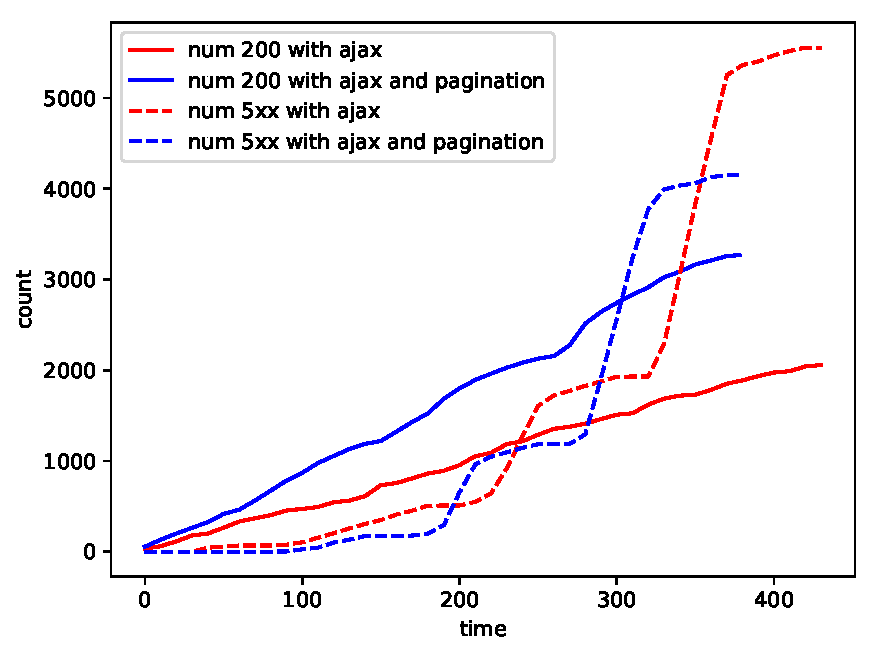
\includegraphics[width=0.46\textwidth]{images/num-code-with-ajax-with-ajax-and-pagination} }}%
    \qquad
    \subfloat[Mean duration of requests.]{{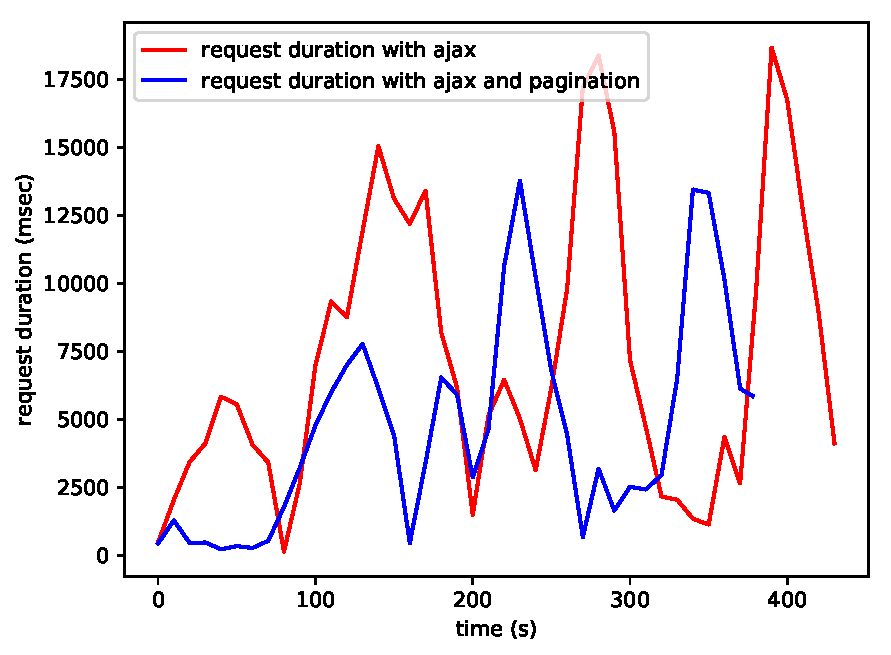
\includegraphics[width=0.46\textwidth]{images/request-duration-with-ajax-with-ajax-and-pagination} }}%
    \caption{Metrics for ajax only and ajax along with pagination.}%
    \label{fig:aap}%
\end{figure}

\section{Optimization: Database Indexing}
The data model of our application was complex. There were multiple different types of relations throughout the database. These relations were queried in one way or another in almost every page of the web app. Therefore we decided to index on the foreign keys of most tables. This resulted in a sharp boost in performance. Figure~\ref{fig:dbindex} shows the mean duration for search transaction (second session of generic workflow as discussed in Section~\ref{sec:generic-workflow}) without and with indexing. It can be observed that indexing made the transaction significantly faster.
\begin{figure}
	\centering
	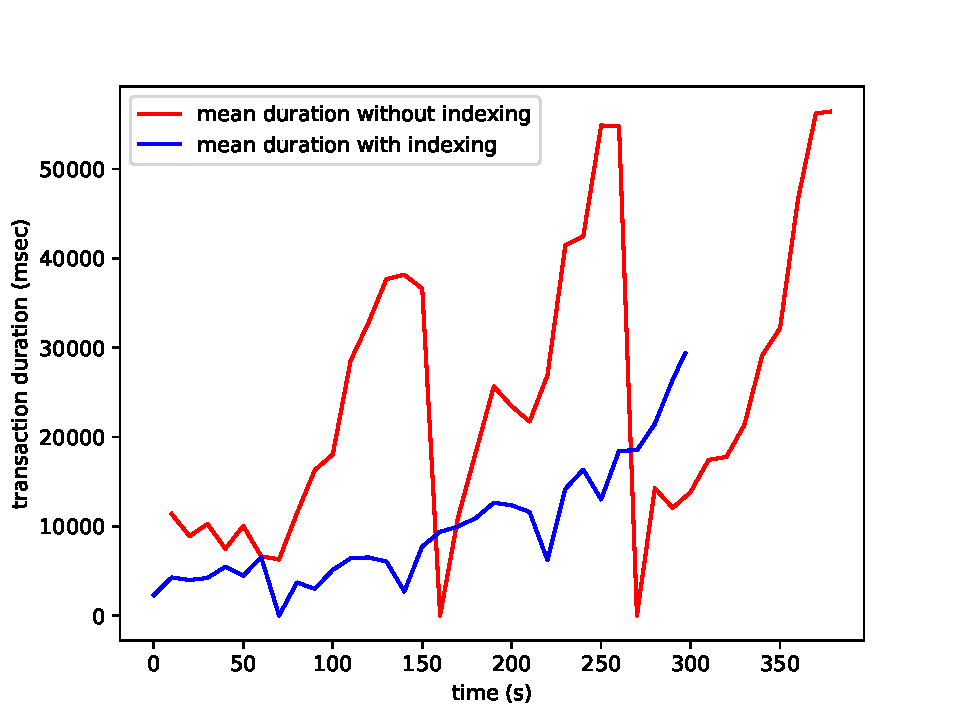
\includegraphics{images/search-transaction-duration-without-indexing-with-indexing}
	\caption{Mean duration for search transaction without and with indexing.}\label{fig:dbindex}
\end{figure}

\section{Optimization: SQL Query}
Careful observation of the Rails log during development revealed that the ``N + 1'' problem of SQL query was prevalent in our application. Specifically, the genres and companies index pages shows the number of games under each genre/company. To retrieve this number, $N$ more queries were triggered in the initial version of the app for $N$ genres/companies apart from the one invoked to get all genres/companies. This situation was later remediated so that instead of ``N + 1'' queries only two queries were invoked. Tsung tests were run on the specific workflow to evaluate the improvement in performance. Figure~\ref{fig:sqlopt} shows the graph of mean duration for the transaction without and with indexing. It is evident from the graph that the discussed SQL optimization greatly improved the response time of the application.
\begin{figure}
	\centering
	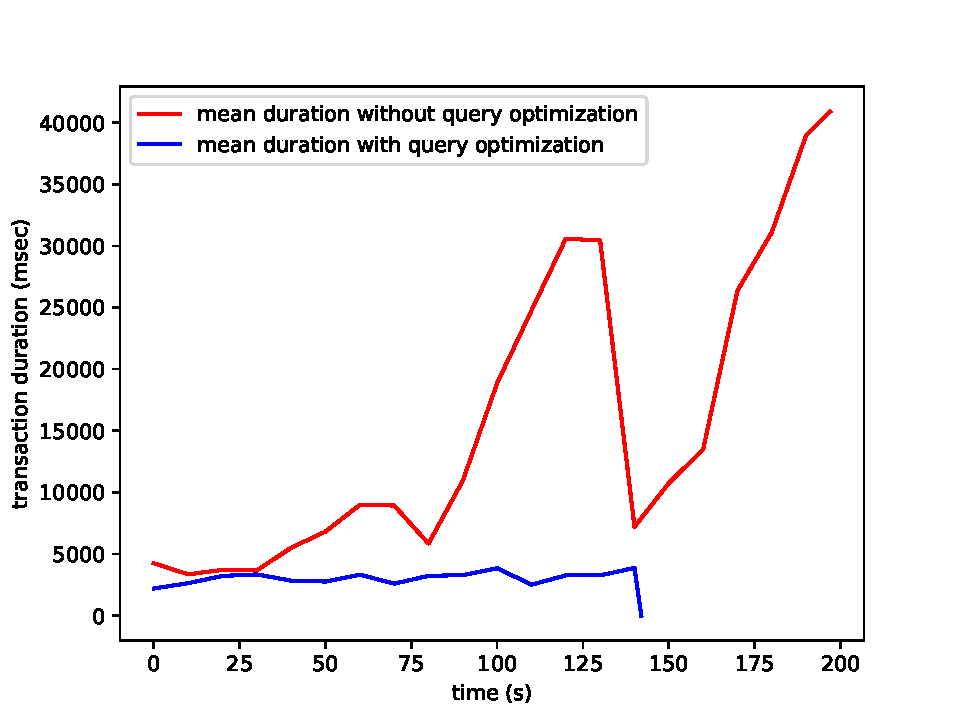
\includegraphics{images/list-pages-transaction-duration-without-query-with-query}
	\caption{Mean duration for index page transaction without and with indexing.}\label{fig:sqlopt}
\end{figure}

\section{Optimization: Caching}
\section{Scaling}
Once all the feasible optimizations were applied to our website, we ran Tsung load-test to obtain the ideal combination of hardware in AWS Elastic Beanstalk. The goal of this exercise was to determine the hardware (app server and database server) combination that was able to handle increasing number of users without producing server-related errors. We varied the number of a particular type of application server (c5 large) and the instance type of the database server. We ran the same Tsung XML file described in the Generic Workflow section on each of hardware configurations. 

\subsection{Results for up to 16 users/second arrival rate}

In this test, the users arrival rate was modeled in four phases with phase 1 beginning with 2 users/second arrival rate. The arrival rate increased by a factor of 2 during subsequent phases with phase 4 having 16 users arriving per second to carry out the transactions set out in the Tsung XML file. 

We started off with a c5 large app server instance and a m4 large database server instance for this test. This combination yielded a significant number of 5xx errors at the end of the test (2612). In the next run, we increased the number of app server to 3 while keeping the same database server. This combination did not result in any significant improvement as we still had 2421 5xx errors. We then ran the test with 10 app servers (maintaining the same database instance type) and interestingly enough noticed a spike in the number of 5xx (2610). This result made it apparent that the true bottleneck of our website is in the database. To solve the problem, we tried a combination of 2 instances of a c5 large app server and m4.4xlarge database instance type. This was the hardware mixture that produced no 5xx error. This test also highlighted the delicate balance that exists between horizontal and vertical scaling. Figure 3.8 shows the mean response time that was achieved by different hardware configurations we tried during this test. From this figure,w e can see that apart from the ideal hardware combination, the other combinations took longer time on average to complete a request made by a user once the arrival rate increased.

\begin{figure}[h]
	\centering
	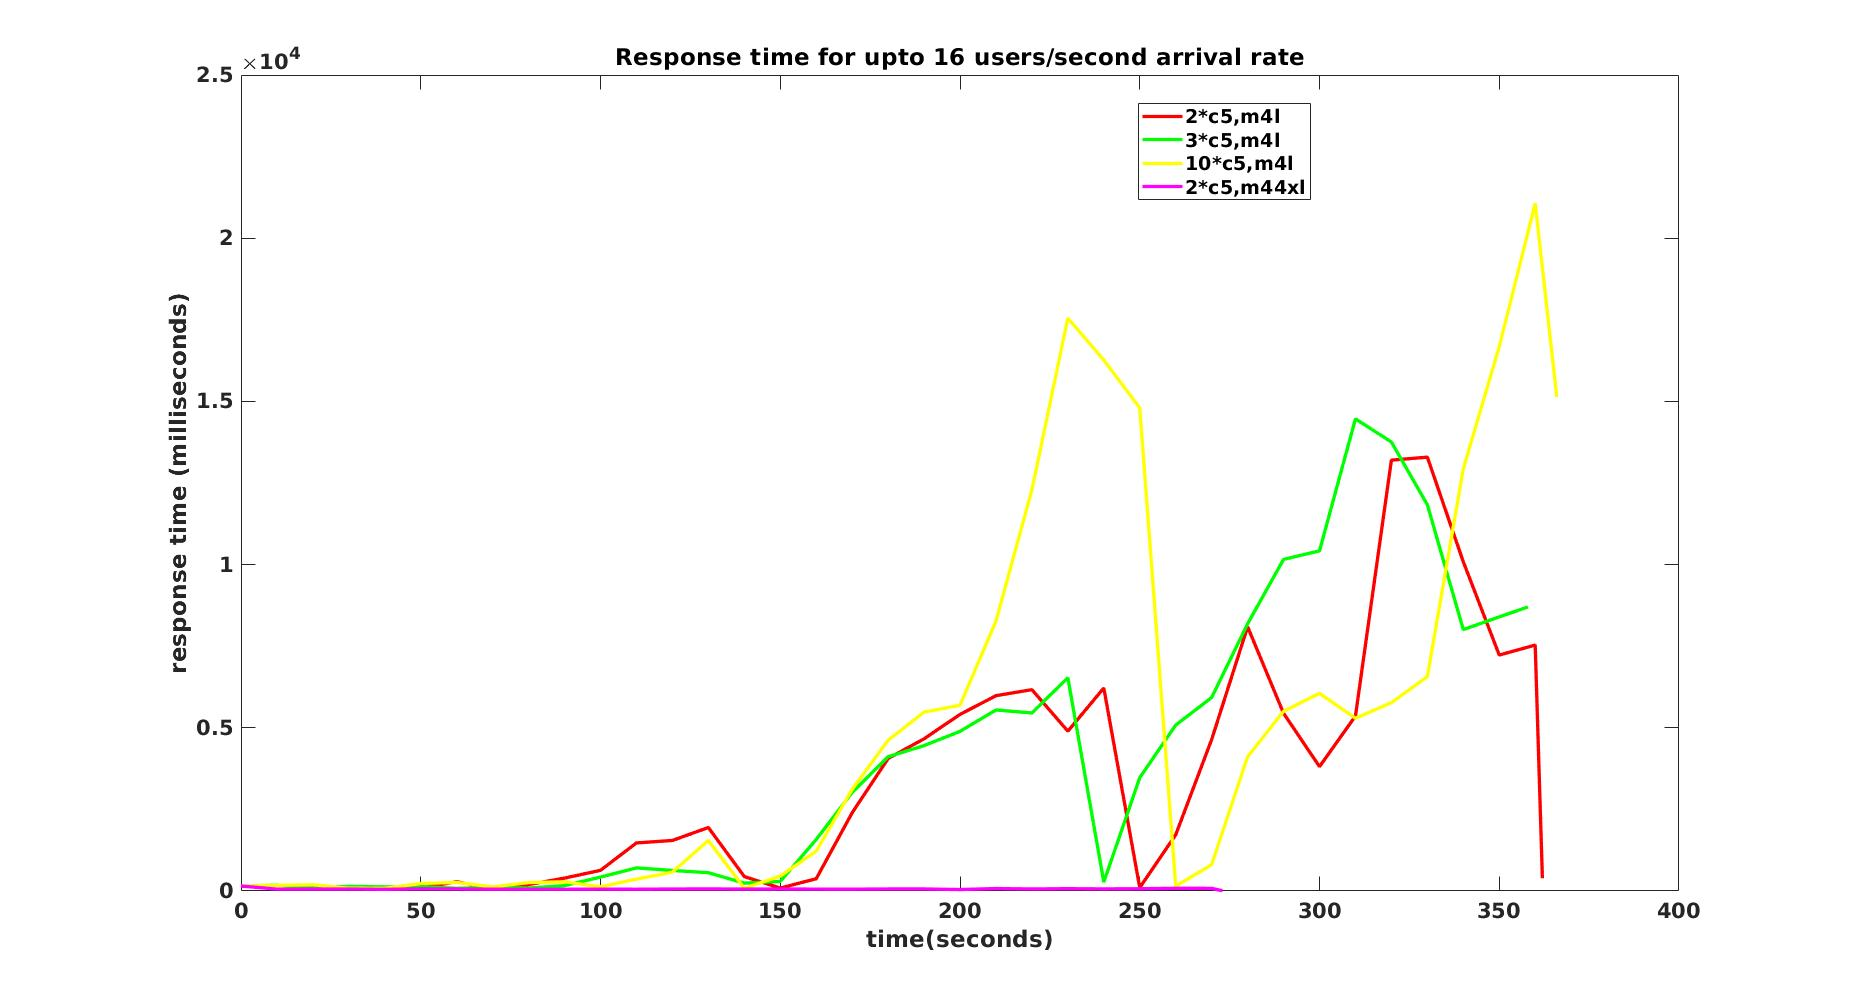
\includegraphics[width=1\textwidth]{images/scale16.jpg}
	\caption{Mean response time while handling up to 16 users/second}\label{fig:sqlopt}
\end{figure}

\subsection{Results for up to 32 users/second arrival rate}
 The users' arrival rate was increased up to 32 per second for this test. We started by keeping the exact hardware combination that produced the best result while handling arrival rate of up to 16 users/second (2 instances of c5.large and a m4.4xl database instance). This combination resulted in 201 5xx errors. Before getting a bigger database instance, we tried to horizontally scale the app server to 4 instances of c5.large. The combination of 4 c5.large app server instances and a m4.4xlarge database server was able to complete the test without resulting in any 5xx errors. Horizontal scaling worked perfectly for this test to be able to handle 32 users/second.
 Figure 3.9 shows the mean response time that was achieved by the two different hardware configurations we tried during this test. It can be observed from this figure that the horizontal scaling resulted in pages being rendered to users much quicker than the combination that produced some number of 5xx errors. 

\begin{figure*}[h]
	\centering
	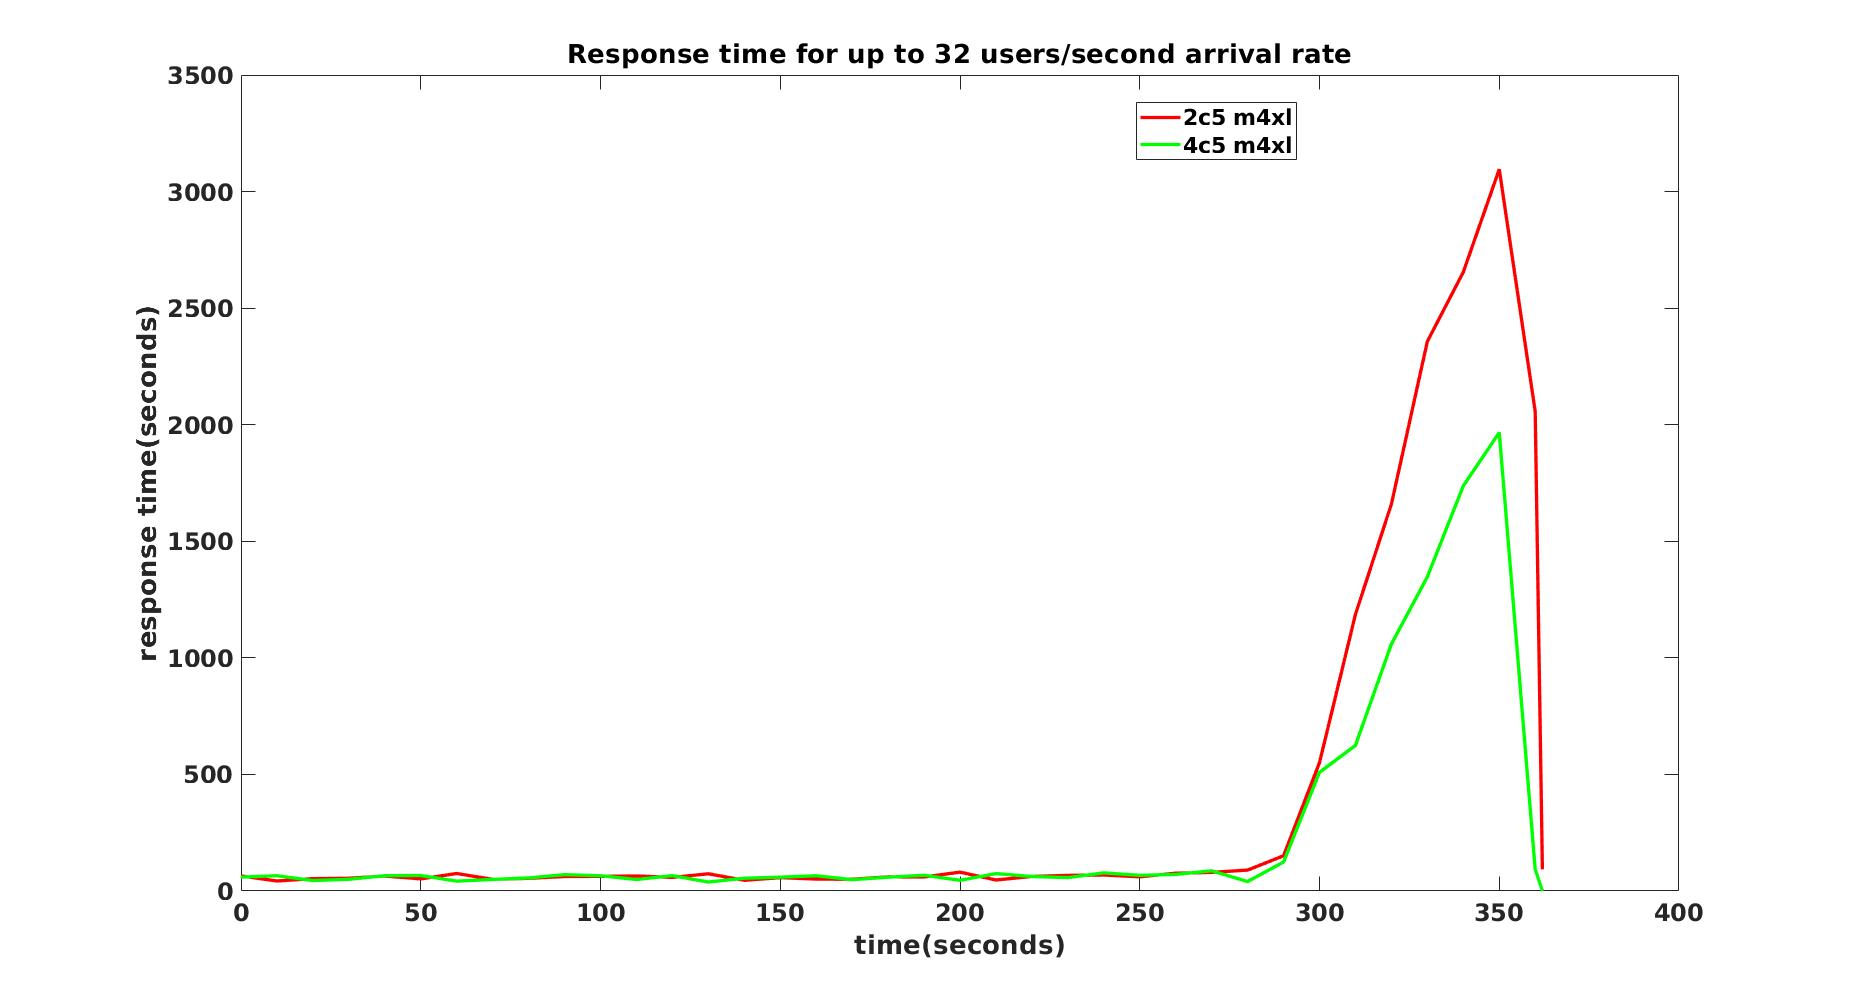
\includegraphics[width=1\textwidth, height=0.5\textheight]{images/scale32.jpg}
	\caption{Mean response time while handling up to 32 users/second}\label{fig:sqlopt}
\end{figure*}


\subsection{Results for up to 64 users/second arrival rate}
We increased the arrival rate by two fold from the previous test to test our website. This test contained 4 arrival phases with the last one having user arrival rate of 64 users/second.  

The test was started with the hardware combination of 4 instances of c5.large application server with a m4.4xlarge database server. This combination produced a total of 5500 5xx error. We followed this by first increasing the number of app servers to 6 and then 8. As the 5xx errors remained, we used a different type of database server instance (m4.10xlarge) with 8 instances of c5.large app server instances. This setting produced no 5xx errors while being able to handle up to 64 users/second. Figure 3.10 demonstrates the mean response time obtained for each combination of hardware we applied during this test. Just as in previous test cases, we can notice that the combination that yielded with no 5xx error was able to meet user generated requests much quicker as opposed to other combinations of hardware. An interesting trend is observed when we horizontally scaled the app server from 6 instances of c5.large to 8 instances. Even though we noticed a decrease in 5xx errors from the former, the latter actually took, on average, longer time to fulfill user requests. This potentially demonstrates that, aside from increased cost, adding more instances does not always produce desired result.

\begin{figure*}[h]
	\centering
	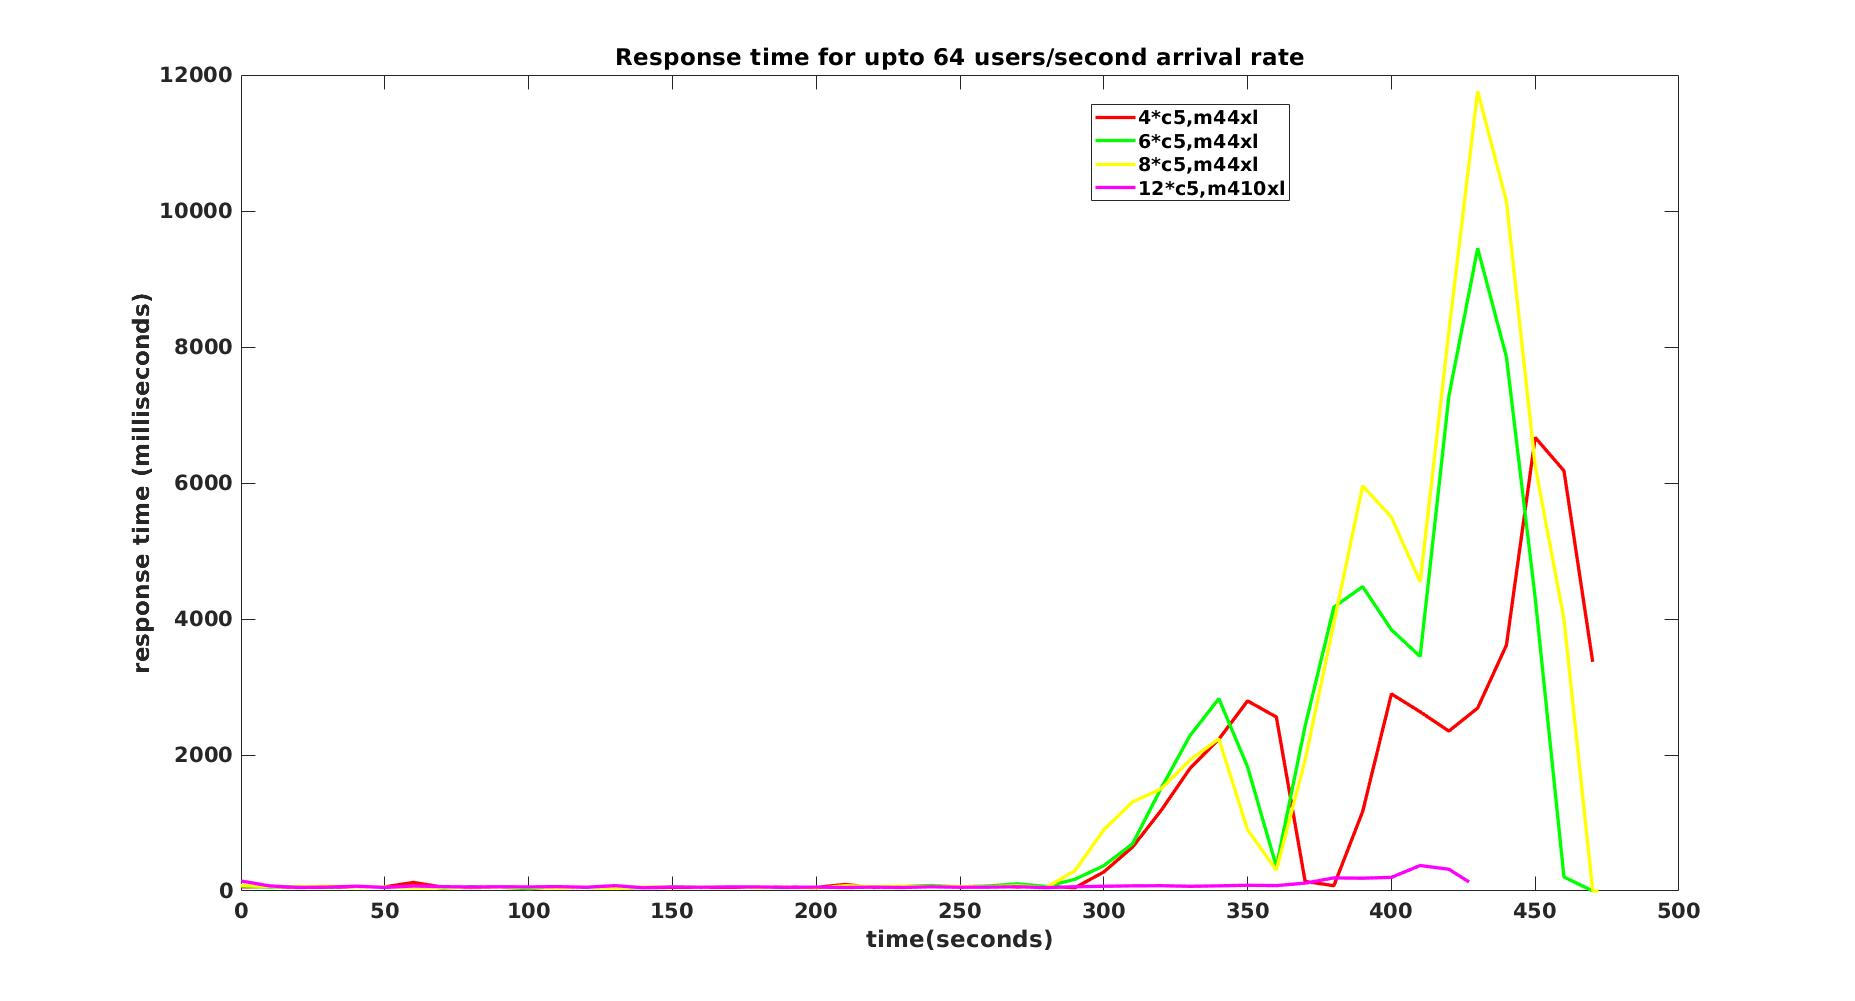
\includegraphics[width=1\textwidth, height=0.5\textheight]{images/scale64.jpg}
	\caption{Mean response time while handling up to 64 users/second}\label{fig:sqlopt}
\end{figure*}


\subsection{Results for up to 128 users/second arrival rate}
The arrival rate was increased to 128 users/second for this test. The first hardware combination used were 8 instances of c5.large app server and m4.10xlarge database server instance. This combination failed to handle the increased number of arrival rate. Subsequently,we tried 10 and 12 instances of c5.large app servers with m4.16xlarge database server instance. The ideal combination for this test that resulted in no 5xx errors were 12 instances of c5.large app server instances and m4.16xlarge of a database instance. Figure 3.11 shows the mean response time each of these combination was able to provide during this test. Here too we can observe that the best combination was able to meet user request in much better time than other combinations.

\begin{figure*}[h]
	\centering
	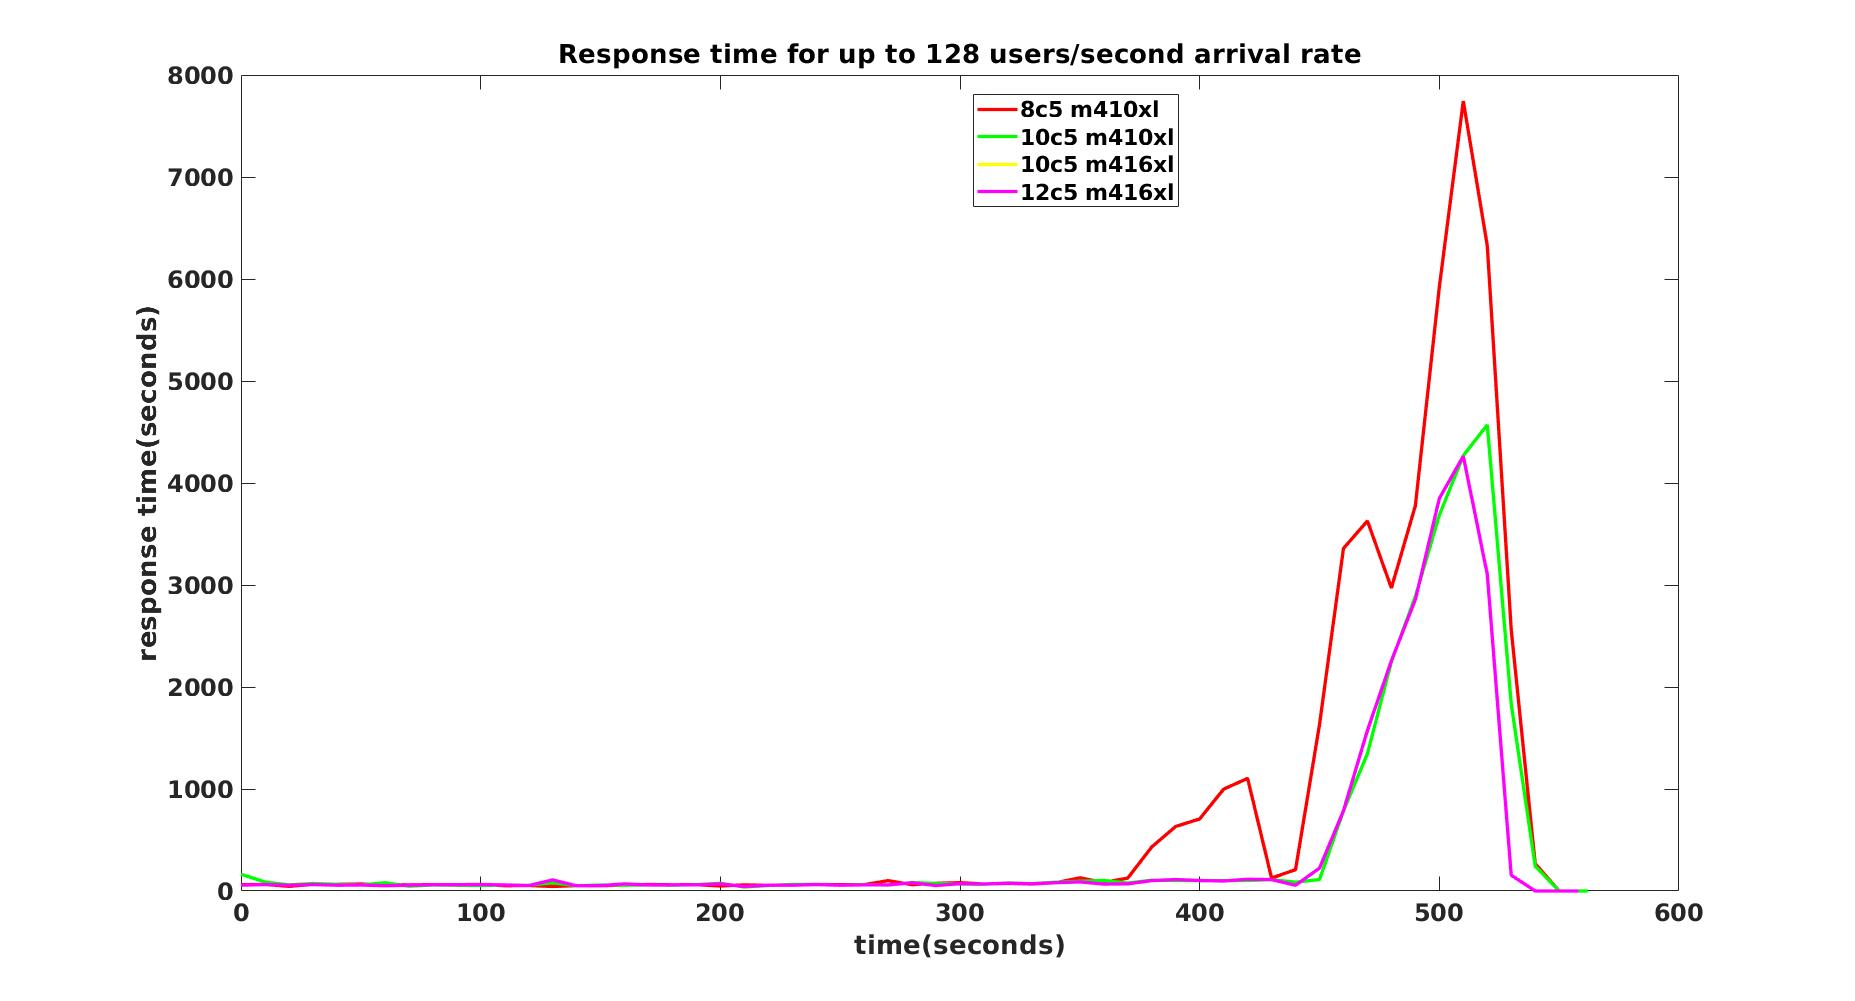
\includegraphics[width=1\textwidth, height=0.5\textheight ]{images/scale128.jpg}
	\caption{Mean response time while handling up to 128 users/second}\label{fig:sqlopt}
\end{figure*}



\subsection{Results for up to 256 users/second arrival rate}
In this test we attempted to determine the hardware combination that could adequately handle 256 users/second arrival rate. In the beginning, We started with 12 instances of c5.large and a ,4.16xlarge app and data base server respectively. This fell well short of meeting the set arrival rate. To tried adding 2 additional app servers but that did not succeed as well. Finally we tried the m5.24xlarge database instance type with 14 instances of c5 large app server. This resulted in only $6\%$ of 5xx errors. At this point, we attempted to utilize a different app server to see if we could overcome the barrier all together. However, our attempt to use the c5d.18xlarge app server did not succeed as the instance failed to properly load up. Figure 3.12 shows the mean response times that were noticed during the different hardware combinations we attempted for this test. From figure, we can conclude that to meet with 256 user requests per second, we need a hardware configuration closer to 14 instances of c5.large app server and a m5.24xlarge database server.

\begin{figure*}[h]
	\centering
	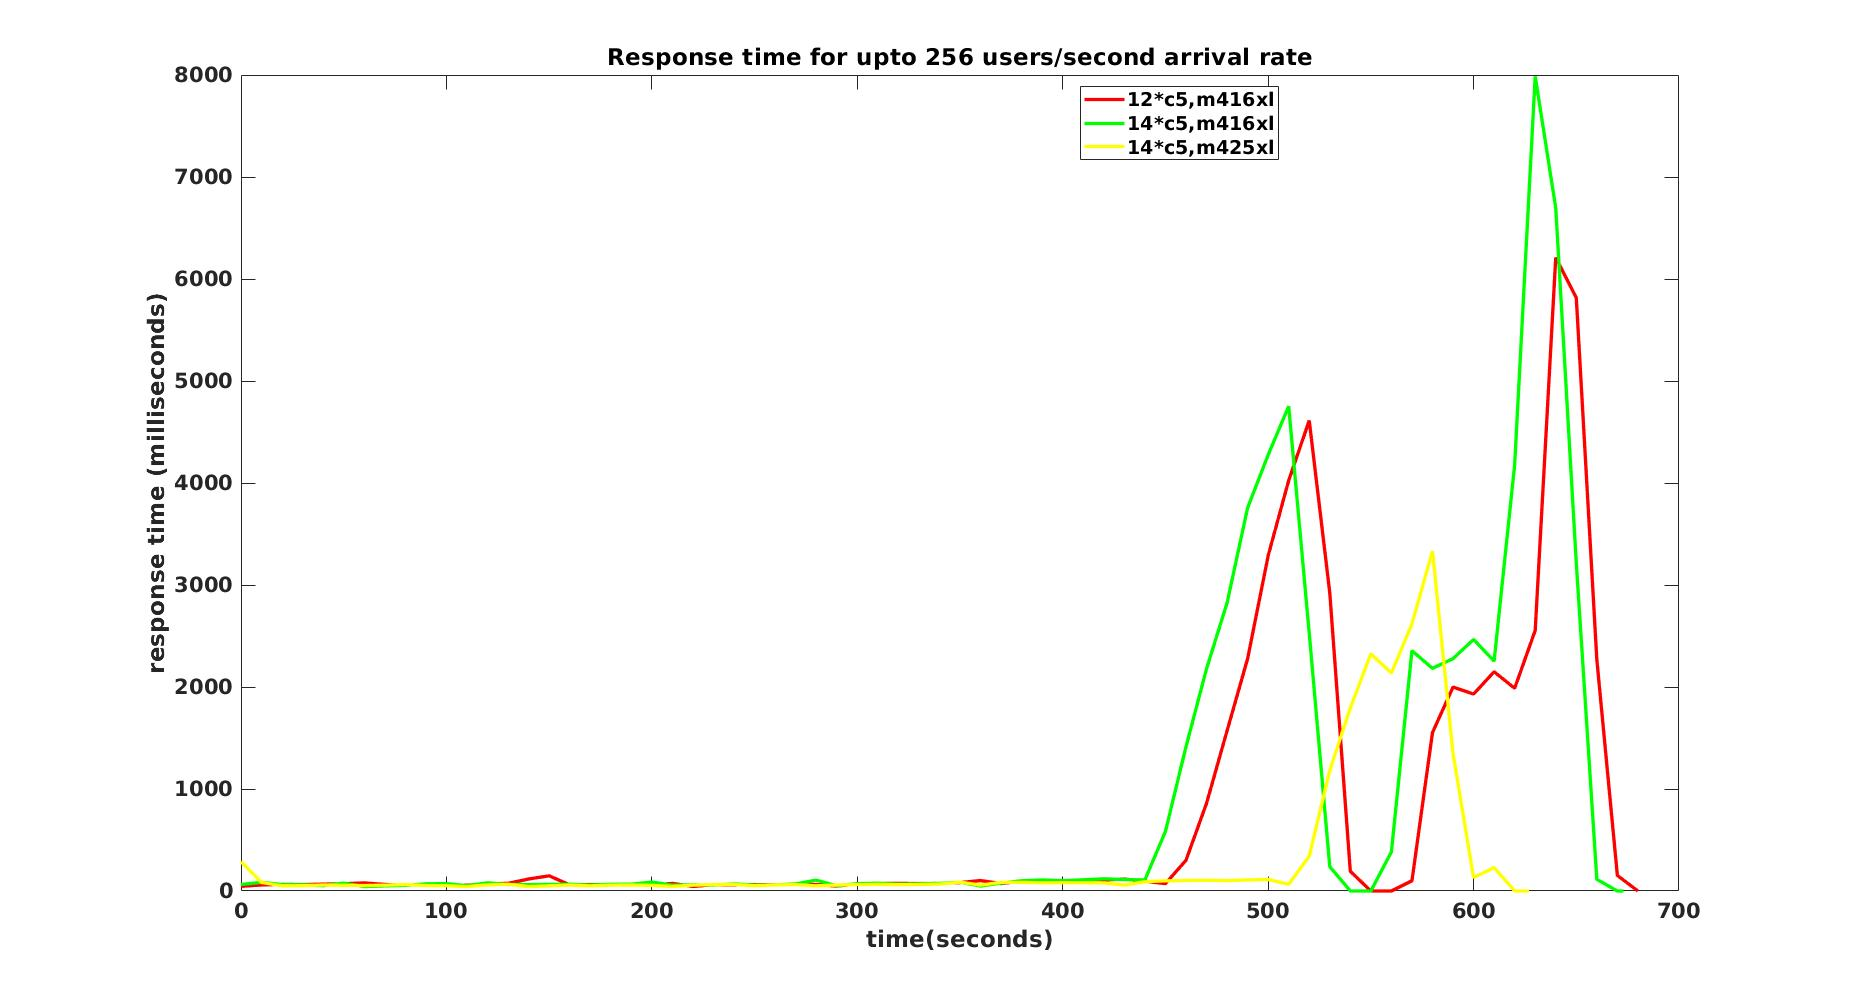
\includegraphics[width=1\textwidth]{images/scale256.jpg}
	\caption{Mean response time while handling up to 256 users/second}\label{fig:sqlopt}
\end{figure*}

\subsection {Cost Benefit Analysis}

Figure 3.13 shows the combination of the hardware that yielded the best result for different number of users' arrival rates per second. This figure also demonstrates the daily cost associated with using each of this hardware combination, thereby easing the process of computing the cost of supporting a certain number of user at any second. Each of these hardware combinations was able to complete the Tsung load test without producing any 5xx HTTP error responses. For example, to meet up with 128 users per second (which could happen during peak time), the hardware combination of 12 c5.large app server instances with a m4.16xlarge database instance is seen to perform best. This combination cost about 7 USD per hour. On the other hand, we can see from Figure 3.13 that to meet up with 32 users/second, we only need to spend around 3 USD. Using tis information, we can be better prepared to handle various levels of users' arrivals during different times of the day.
\begin{figure*}[h]
	\centering
	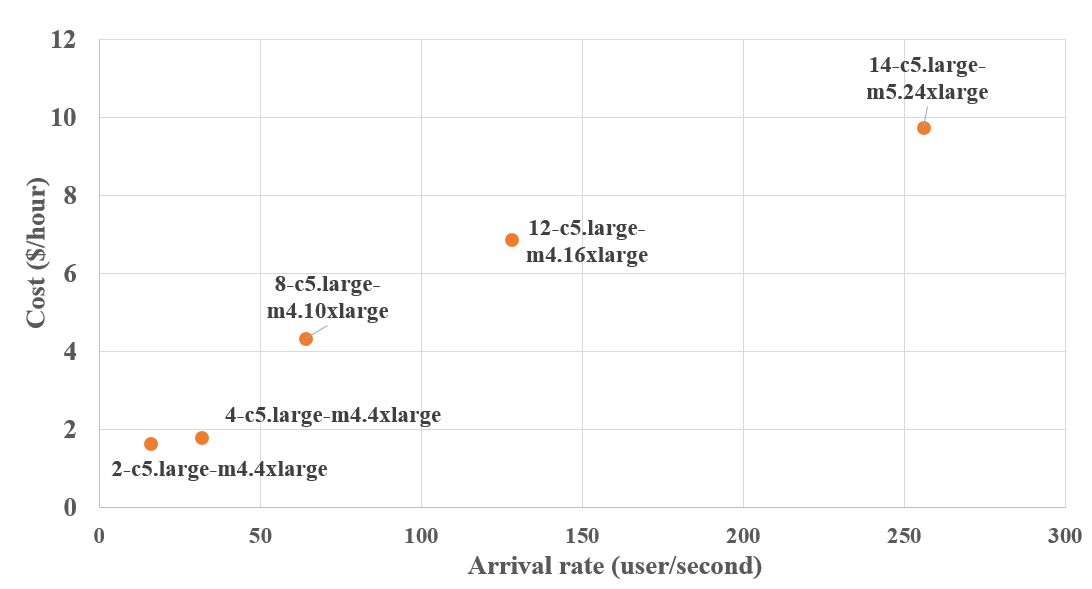
\includegraphics[width=1\textwidth]{images/cost.PNG}
	\caption{Cost against user arrival rate for different AWS hardware configurations}\label{fig:sqlopt}
\end{figure*}


